%%% Local Variables: 
%%% mode: latex
%%% TeX-master: "../thesis"
%%% End: 

\section{Introduction}
\label{sec:probobj_introduction}
Dense SLAM (Simultaneous Localisation and Mapping) has proven to be an effective
paradigm for the reconstruction of scenes of moderate size, with much research
on the topic driven by the availability of consumer grade depth sensing
equipment. However, there is a heavy reliance on descriptive geometry in the
scene when there is a lack of texture. Less descriptive geometry leads to an
increase in camera tracking error and causes model inconsistencies, especially
when a loop closure event occurs.

As object reconstruction can be seen as a smaller scale equivalent of the scene
based dense reconstruction problem, it too is prone to the tracking drift and
loop closure problem, sometimes to a prohibitive level. Often it may be
desirable to perform object reconstruction in an interactive way, for example,
as a component of a scene understanding system, or to procure training data for
the object in question.

With a high level of interaction comes an exacerbation of the aforementioned
shortcomings of dense SLAM, particularly due to the potential for frequent,
repetitive motion. This is the problem that is addressed in this chapter.

In this chapter, a probabilistic object reconstruction framework is presented
for the reconstruction of rigid objects based on object appearances.
The framework facilitates the correction of camera tracking drift by
representing the object to be reconstructed as a collection of overlapping
subsegments, such that deformations may be inferred to keep the subsegments
aligned, resulting in a consistent overall model. The system utilises a
volumetric representation for each of these object subsegments, as with many
larger scale reconstruction systems. Each voxel in the subsegments has
additional appearance posterior information pertaining to the voxels membership
of the object.

Over time, multiple volumes containing both surface and probabilistic appearance
information are maintained and manipulated to yield a robust and temporally
consistent model. Finally, the optimum object shape is optimised for within a
CRF (Conditional Random Field) framework.

The proposed system is inspired by\cite{Kolev2006} in that the representation
used for the shape of the object to be modelled is a volume of probabilities,
pertaining to posteriors over a voxels assignment to being either on the objects
surface or not. In the proposed system this volume of posterior probabilities is
``fused'' into with each frame, much like the fusion process in systems such as
KinectFusion\cite{Newcombe2011} and InfiniTAM\cite{Prisacariu2014}.

The probabilities that are ``fused'' into the volume are generated from an
appearance model, initialised prior to reconstruction by a Maximum Likelihood
procedure over the first frame of the RGB image. There are two appearance
models, one for the foreground object and one for the background, with the
foreground object indicated by a bounding box on the first RGB frame. A normal
distribution is fitted over the colour features of each class, foreground and
background. During the fusion process, the PDF's of these distributions are
evaluated on the latest colour observation for a voxel and posterior's are
computed and updated accordingly in the probability volume. Only those voxels
with a posterior higher for the foreground are rendered.

\section{Related Work}
\label{sec:probobj_related_work}

\section{Algorithm Overview}
In the proposed system, the object model is divided into Subvolumes, each
consisting of a TSDF, colour volume and object Probability Volume. Additionally,
each has associated with it a Rigid Body Transform that specifies its pose
relative to the global coordinate frame.

At each time step, a segmentation model is applied to the RGB input image to
generate an object \textit{Probability Map} defining the segmented region to be
the object of interest and the remainder the background, to be discarded. Using
these generated Probability Maps, the system accumulates the probabilities into
the object \textit{Probability Volume} of the active Subvolume.

As with the Dense SLAM system outlined earlier in this work, the proposed system
also has \textit{Integration}, \textit{Tracking} and \textit{Rendering}
stages in it's pipeline(all of which are run at each time step). However, in
the proposed system, there are an additional two stages to the pipeline;
\textit{Online Model Correction} and \textit{CRF Based Segmentation}.

At the end of each frame, the online model correction algorithm is run, which
infers the relative poses between the subvolumes, mitigating tracking drift.
Once the reconstruction process is finished, we perform a CRF-based optimisation
to refine the resulting object segmentation over all Subvolumes.

The proposed approach is not tied to the use of any one probabilistic model,
though in the presented experiments PwP (Pixel Wise Posteriors) are used
\cite{Bibby2008}. An overview of the object reconstruction pipeline is shown in
Figure \ref{fig:probobj_pipeline_diagram}.

\begin{figure}[ht]
  \label{fig:probobj_pipeline_diagram}
  \centering
  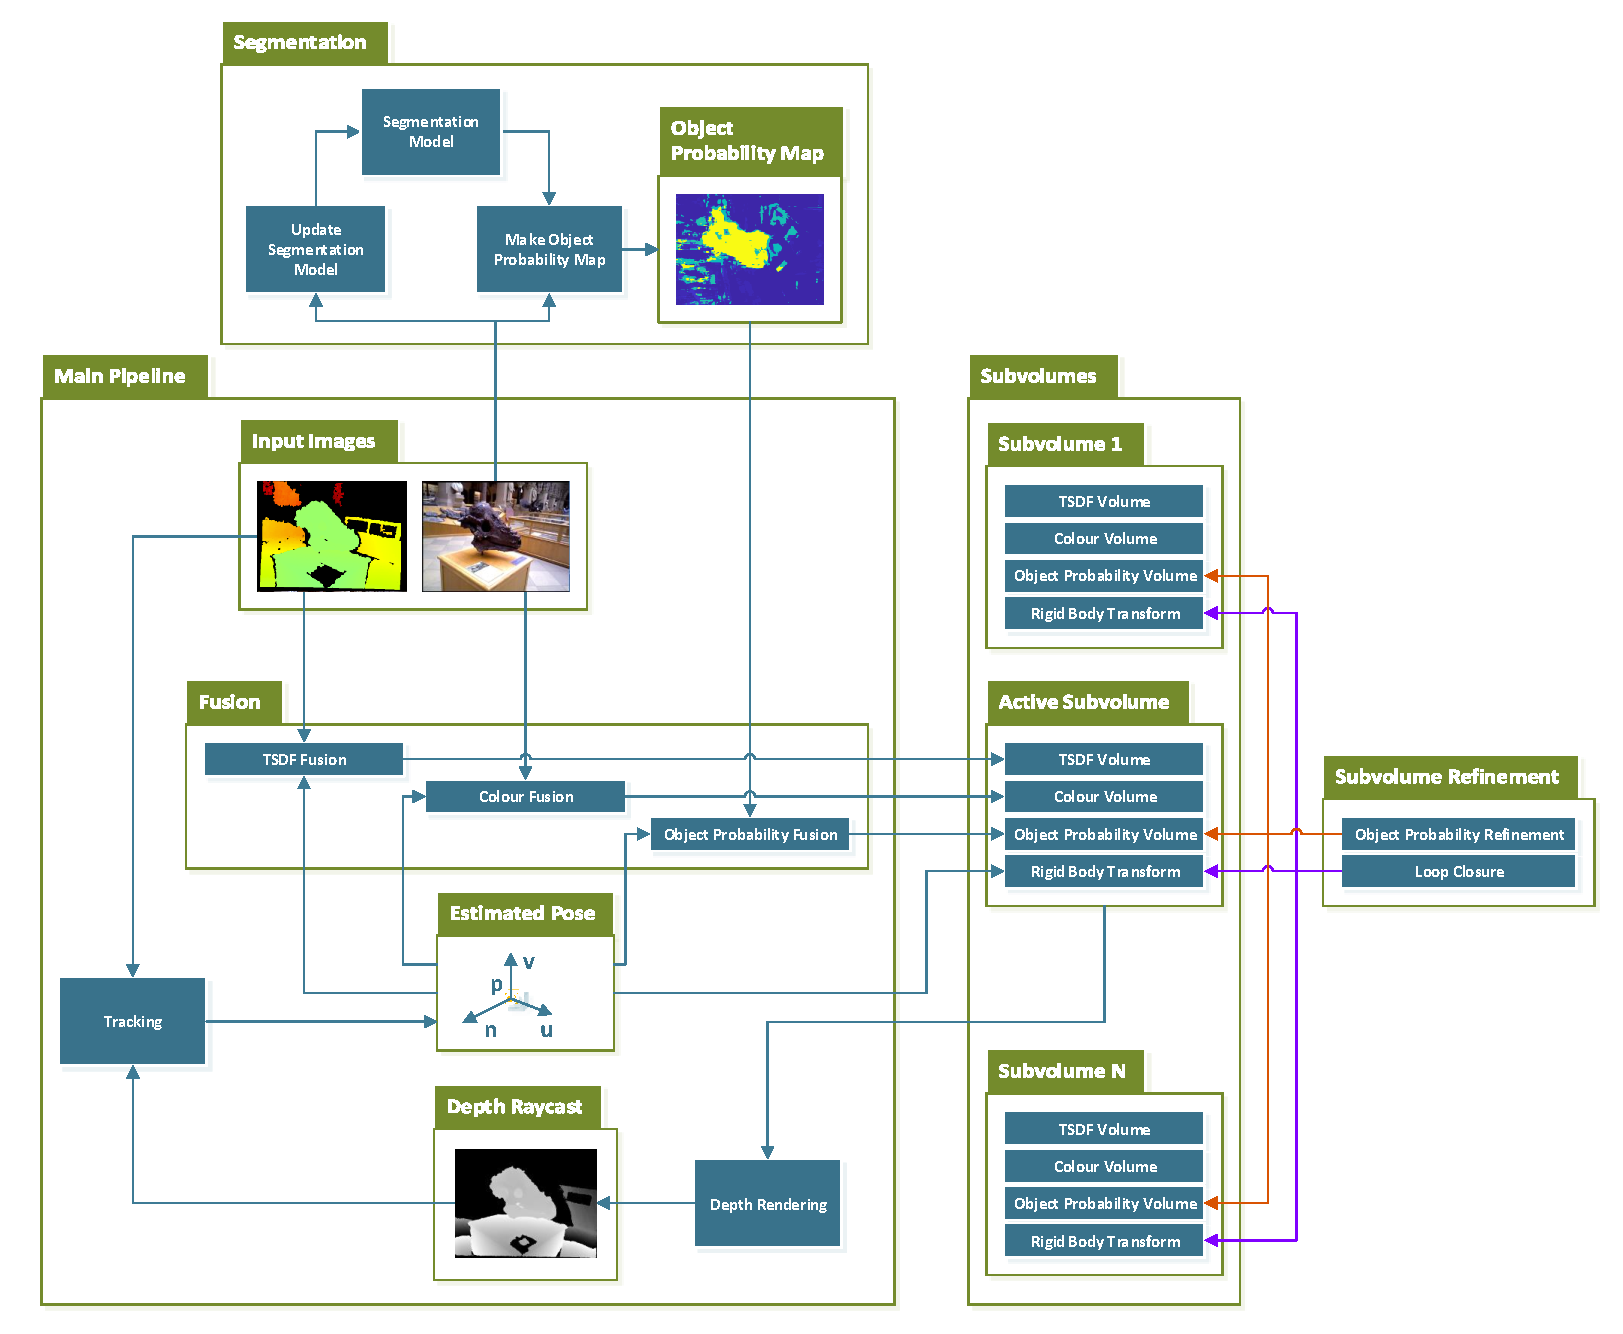
\includegraphics[width=\linewidth]{figures/object_recon/pipeline.pdf}
  \caption{The pipeline of the proposed Object Reconstruction approach.}
\end{figure}

\section{Probabilistic Formulation of Object Reconstruction}
\label{sec:probobj_prob_formulation}
The surface map and camera pose are estimated using the standard KinectFusion
like pipeline of \cite{Newcombe2011,Prisacariu2014}. The surface is represented
as the Zero Level Set of a TSDF discretised over voxels, with the Isosurface
built by a weigted mean of new observations, as outlined in Equations
\ref{eqn:sdf_update} and \ref{eqn:sdf_weight_update}. Camera Pose Estimation is
performed with ICP, as outlined in Section
\ref{subsec:moseg_static_camera_trackin} and is run quasi-simultaneously against
the evolving map. Here, inspired by \cite{Kolev2006}, this procedure is
augmented by estimating the Posterior Probability, per map Voxel, of belonging
to the object of interest. This volume of Posterior Probabilities is updated at
each time step, in parallel to the fusion process in the mapping and pose
estimation components of the Pipeline. The representation of the reconstructed
object comprises multiple ``subvolumes'', each pertaining to some patch on the
object surface. New subvolumes are created when sufficiently many new Voxels
have been allocated and have had SDF data integrated. By ensuring overlap
between the subvolumes, transformations between them can be found and pose
inconsistencies addressed, online. Empirically, the threshold for starting a new
subvolume is defined as the event when $50\%$ of the Voxels fused in to the
current volume are newly observed points.

\subsection{Volumetric Appearance Model}
\label{subsec:probobj_vol_appearance_model}
At each observed RGBD frame, the object Posterior Probabilities for the visible
Voxels in the active submap are updated via an appearance-derived Probability
Map for that frame. Under the assumption of Conditional Independence between
frames (for sake of tractability), the Posterior Probability of a given voxel
$\psi \in \Psi$ belonging to the object has the following form(noting that
$\Phi \subset \Psi$):
\begin{equation}
\label{eqn:probobj_voxel_posterior}
P(\psi \in \Phi | \Omega, p) = \prod_{t=0}^{\infty}
P(\psi_{t} \in \Phi | \Omega_{t}, p_{t})
\end{equation}
where $\Psi$ is the volume of voxels for which measurements are accumulated,
$\Phi$  is the volume of Voxels pertaining to the object, $\Omega_{t}$ is the
current RGBD image observation at time $t$ and $p_{t}$ is the currently tracked
pose at time $t$. This encodes the Probability of a Voxel belonging to the
object of interest as the product of instantaneous appearance-derived pixel-wise
conditionals. Note that in the above, $\Phi$ is a discretisation of the
continuous $\Phi$ in the probabilistic formulation that follows.

\subsection{Full Joint Definition}
\label{subsec:probobj_full_joint}
Central to the proposed system is the aforementioned Volume of appearance based
Posterior Probabilities pertaining to a Voxel wise membership of either the
object Voxel set or the non object(background) Voxel set. This allows
formulation of the full joint distribution over the object as the Probabilistic
Graphical Model of Figure \ref{fig:pgm}.

\begin{figure}[ht]
  \label{fig:probobj_pgm1}
  \centering
  \resizebox {0.4\linewidth}{!}{
    \begin{tikzpicture}
      % Declare nodes.
      \node[latent] (phi) {$\Phi$};
      \node[latent, right=of phi] (u) {$u$};
      \node[latent, below=of u] (L) {$L$};
      \node[obs, right=of u, yshift=-1cm] (omega) {$\Omega$};
      \node[obs, right=of u, yshift=1cm] (p) {$p$};
      
      % Setup plates.
      \plate[inner sep=0.25cm] {plate1} {(omega) (p)} {t, p};
      \plate[inner sep=0.25cm] {plate2} {(u) (phi)} {$\Psi$};
      \plate[inner sep=0.25cm] {plate3} {(L)} {s, s'};
      
      % Setup edges.
      \edge {omega, p} {u, L}
      \edge {L} {phi}
      \edge {u} {phi}
    \end{tikzpicture}
  }
  \caption{Probabilistic Graphical Model representing the full Joint
    Distribution over the shape $\mathbf{\Phi}$ of the object of interest.}
\end{figure}

Where $\Phi$ is the shape of the object to be reconstructed (represented as a
subset of Voxels for which surface data has been Integrated into the relevant
TSDF), $u$ is the appearance model volume(aforementioned appearance Posteriors),
$L$ is the set of consistency constraints for each adjacent sub volume pair in
the form of Rigid Transformations, $\Omega$ is the set of RGBD image pixels and
$p$ the set of poses over time.

The PGM given in Figure \ref{fig:probobj_pgm1} leads to the following
factorisation over the full Joint Distribution.
\begin{equation}
  \label{eqn:probobj_full_joint}
  P(\Phi, \Omega, p, u, L) = 
  \prod_{\psi \in \Psi}\prod_{s, s' \in \mathcal{S}}
  P(\Phi \given u_{\psi}, L_{s, s'}) 
  \prod_{t=0}^{\infty}\prod_{p \in \mathcal{P}}
  P(u_{\psi} \given \Omega_{p, t}, p_{t})
  P(L_{s, s'} \given \Omega_{p, t}, p_{t})
  P(L_{s, s'})P(p_{t})P(\Omega_{p, t})
\end{equation}
Where in Equation \ref{eqn:probobj_full_joint}, $\Psi$ is the set of Voxels
across all subvolumes, $\mathcal{P}$ is the set of RGBD pixels for a given 
frame and $\mathcal{S}$ is the set of subvolumes. Note that the notation
$s, s' \in \mathcal{S}$ refers to pairs of overlapping subvolumes.

If pixel-wise independence is assumed in the RGBD observations and temporal
independence is assumed in the poses, the plate containing $\Omega$ and $p$ can
be removed as shown in Figure \ref{fig:probobj_pgm2}.
\begin{figure}[ht]
  \label{fig:probobj_pgm2}
  \centering
  \resizebox {0.4\linewidth}{!}{
    \begin{tikzpicture}
      % Declare nodes.
      \node[latent] (phi) {$\Phi$};
      \node[latent, right=of phi] (u) {$u$};
      \node[latent, below=of u] (L) {$L$};
      \node[obs, right=of u, yshift=-1cm] (omega) {$\Omega$};
      \node[obs, right=of u, yshift=1cm] (p) {$p$};
      
      % Setup plates.
      \plate[inner sep=0.25cm] {plate3} {(L)} {s, s'};
      \plate[inner sep=0.25cm] {plate2} {(u) (phi)} {$\Psi$};
      
      % Setup edges.
      \edge {omega, p} {u, L}
      \edge {L} {phi}
      \edge {u} {phi}
    \end{tikzpicture}
  }
  \caption{Probabilistic Graphical Model representing the simplified Joint
    Distribution over the shape $\mathbf{\Phi}$ of the object of interest.}
\end{figure}

The simplifications transforming the PGM of Figure \ref{fig:probobj_pgm1} in to
that of Figure \ref{fig:probobj_pgm2} lead to the following Factorisation of the
Joint Distribution over $\mathbf{\Phi}$.
\begin{equation}
  \label{eqn:probobj_simplified_joint}
  P(\Phi, \Omega, p, u, L) = 
  \prod_{\psi \in \mathbf{\Psi}}P(\Phi \given u_{\psi})
  \prod_{s, s' \in \mathcal{S}}P(u_{\psi} \given \Omega, p, L_{s, s'})
  P(L_{s, s'} \given \Omega, p) P(L_{s, s'})P(p)P(\Omega)
\end{equation}

The formalisms defined in Figures \ref{fig:probobj_pgm1} and
\ref{fig:probobj_pgm2} and Equations \ref{eqn:probobj_full_joint} and
\ref{eqn:probobj_simplified_joint} describe a probabilistic framework in which
online corrections can be made to the reconstructed model(piecewise over
subvolumes) to counter errors caused by pose tracking inconsistencies. As with
scene scale dense SLAM systems\cite{Newcombe2011, Prisacariu2014, Niessner2013},
the presented system follows a pipeline that consists of a tracking stage and an
integration stage, as outlined in Section \ref{sec:moseg_static_fusion}.

However, the presented formulation of this pipeline consists of an
additional, novel estimation module that relies on the use of a subvolume
representation to correct tracking errors by applying Rigid Body Transformations
to the subsegments of the reconstructed shape(the subvolumes) to correct their
alignment when there are intra subsegment tracking inconsistencies. As inference
on the Joint Distribution of the presented Probabilistic Model model is
intractable, Conditional Independence assumptions are made that empirically do
not appear to cause any functional issues.

\subsection{Appearance Marginal}
Continuing on from the formulation given in Equation
\ref{eqn:probobj_simplified_joint}, the appearance model $u$ may be Marginalised
as follows.
\begin{align}
  \label{eqn:probobj_appearanc_marginal}
  % Line 1.
  P(\Phi, \Omega, p, L) & =
  \int_{-\infty}^{\infty} \Bigg[ 
  \prod_{\psi \in \mathbf{\Psi}} P(\Phi \given u_{\psi})
  \prod_{s, s' \in \mathcal{S}}P(u_{\psi} \given \Omega, p, L_{s, s'})
  P(L_{s, s'} \given \Omega, p) P(L_{s, s'})P(p)P(\Omega) \Bigg] \intd{u} \\
  % Line 2.
  & = \prod_{\psi \in \mathbf{\Psi}} 
  \int_{-\infty}^{\infty} \Bigg[ P(\Phi \given u_{\psi})
  \prod_{s, s' \in \mathcal{S}}P(u_{\psi} \given \Omega, p, L_{s, s'})
  P(L_{s, s'} \given \Omega, p) P(L_{s, s'})P(p)P(\Omega) \Bigg] \intd{u} \\
  & = \prod_{s, s' \in \mathcal{S}} P(L_{s, s'} \given \Omega, p)
  P(L_{s, s'})P(p)P(\Omega)P(\mathbf{\Phi})
\end{align}
Note that the Appearance Posterior Volume outlined in Section 
\ref{subsec:probobj_vol_appearance_model} is reintroduced later in this work in
Section \ref{} for the purposes of subvolume alignment and determining the
subset of Voxels $\mathbf{\Phi} \subset \mathbf{\Psi}$ that determine the target
object shape.

Further details pertaining to the inference procedure for the per-subvolume
deformations is provided in Section \ref{sec:probobj_model_correction}.

\section{Online Model Correction}
\label{sec:probobj_model_correction}
The tracking consistency constraints denoted by the variables $L_{s, s'}$ such
that $s, s' \in \mathcal{S}$ with $\mathcal{S}$ being the set of overlapping
subvolume pairs $s, s'$ in the Probabilistic Graphical Models given by Figures
\ref{fig:probobj_pgm1} and \ref{fig:probobj_pgm2} can be enforced in terms of
minimising the disparity between each pair of adjacent subvolumes. The effect of
this minimsation being that consistency in the Pose Estimation phase of the
Pipeline outlined in Figure \ref{fig:probobj_pipeline_diagram} is enforced. The
objective of this procedure is to infer a robust and consistent deformation
transformation for the subvolume pair.

\subsection{Alignment MAP Estimate}
\label{subsec:probobj_alignment_map}
Referring back to the joint distribution of Equation
\ref{eqn:probobj_simplified_joint}, to achieve the aforementioned minimisation
of disparity between overlapping subvolumes, a Maximum a Posteriori (MAP)
estimate is desirable. As such, a MAP estimate over $L_{s, s'}$ in Equation
\ref{eqn:probobj_simplified_joint} for a given subvolume pair $s, s'$ may be
derived as follows.
\begin{align}
  \label{eqn:probobj_map_estimate}
  % Line 1.
  P(\Omega, p | L_{s, s'}) & \propto \prod_{s, s' \in \mathcal{S}}
  \frac{P(L_{s, s'} | \Omega, p) 
  P(\Omega | p)P(p)P(L_{s, s'})}
  {\displaystyle\int_{-\infty}^{\infty} P(L_{s, s'} \given \Omega, p)
  \intd{L_{s, s'}}} P(\Phi) \\
  % Line 2.
  & \propto \prod_{s, s' \in \mathcal{S}} P(L_{s, s'} | \Omega, p) P(\Omega | p)
  P(p)P(L_{s, s'})P(\Phi) \\
  % Line 3.
  & \propto \prod_{s, s' \in \mathcal{S}} P(L_{s, s'} | \Omega, p)P(L_{s, s'})
  P(\Phi)
\end{align}
Note that in the third step of Equation \ref{eqn:probobj_map_estimate} the
distributions $P(\Omega | p)$ and $P(p)$ are taken to be Uniform and as such may
be omitted whilst retaining proportionality. The distribution $P(L_{s, s'})$ is
Conjugate to $P(L_{s, s'} | \Omega, p)$ and is of the form of a Multivariate
Gaussian Distribution $\mathcal{N}(\mathbf{0} \given \mathbf{I})$ over the
$\mathbb{SE}(3)$ deformation parameters. The choice of such a Prior Distribution
is motivated by the assumption that motion between consecutive frames is minor,
thus the given Prior will have the effect of constraining the $\mathbb{SE}(3)$
transformation as such. The Prior distribution $P(\Phi)$ serves as a
\textit{Surface Prior} to mitigate the effect of noise introduced in to the TSDF
volumes. The form of $P(\Phi)$ shall be discussed in Section
\ref{subsec:probobj_analytic_alignment_map}.

The rationale of Equation \ref{eqn:probobj_map_estimate} is that the deformation
$L_{s, s'}$ applied to the subvolume $s$ maximises the Posterior Probability of
observing the current pose $p$ given the current RGBD frame $\Omega$ by reducing
the variance of the result of the Pose Estimation phase of the Pipeline. As such,
global tracking variance (quantified by the proportion of outliers in the result
of the ICP component of the Pipeline) is reduced by enforcing local consistency,
also improving global consistency and thus the quality of the resultant
reconstruction.

\subsection{Analytic Form of Alignment MAP Estimate}
\label{subsec:probobj_analytic_alignment_map}
With the Probabilistic framework now outlined, the analytic form of the
Posterior given in Equation \ref{eqn:probobj_map_estimate} may be explored. The
Likelihood term in Equation \ref{eqn:probobj_map_estimate} quantifies the
ability of the constraint $L_{s, s'}$ to maximise consistency between subvolumes
$s$ and $s'$, with respect to observed RGBD Frame $\Omega$ and Pose $p$. By
quantifying the Likelihood only for Voxels in $s$ and $s'$ that are visible in
the current view frustrum at time $t$, the Posterior $P(\Omega, p | L_{s, s'})$
is given. As outlined in Section \ref{subsec:probobj_alignment_map}, the Prior
on the constraints $L_{s, s'}$ has the form of a Multivariate Gaussian
Distribution of the form $\mathcal{N}(\mathbf{0}, \mathbf{I})$.

As such, the analytic form of the Likelihood term $P(L_{s, s'} | \Omega, p)$ is
given as follows.
\begin{equation}
  \label{eqn:probobj_likelihood_analytic}
  P(L_{s, s'} | \Omega, p) = \prod_{(s, s') \in \mathcal{S}}
  \frac{1}{\sqrt{2 \pi \sigma}}
  \exp{\frac{-\big(\Phi_{s}(\mathbf{x}) -
  \Phi_{s'}(\Lambda(\mathbf{x}, \mathbf{p}, \mathbf{t}))\big)^{2}}
  {2\sigma^{2}}}
\end{equation}

In Equation \ref{eqn:probobj_likelihood_analytic}, the function $\Lambda(.)$
applies the resultant $\mathbb{SE}(3)$ Transform to a given Voxel position
$\mathbf{x}$ and is defined as follows.
\begin{equation}
  \label{eqn:probobj_lambda_fn}
  \Lambda(\mathbf{x}, \mathbf{p}, \mathbf{t}) =
  \mathbf{R}_{\mathbf{p}} \mathbf{x} + \mathbf{t}
\end{equation}
In Equation \ref{eqn:probobj_lambda_fn} $R_{\mathbf{p}}$ is the $\mathbb{SO}(3)$
Rotation Matrix generated from the Rodrigues Parameters given by the Vector
$\mathbf{p}$. Recall the definition of the Rodrigues Paramaterisation given in
Equation \ref{eqn:rodriguez_matrix_eq} of Section
\ref{subsub:moseg_static_camera_attitude}.

The form of the aforementioned Surface Prior $P(\Phi)$ is taken to be that of
the Logistic Distribution, due to the ``symmetric'' $1 - f(x) = f(-x)$
and ``squashing'' $\text{Range}[f(x)] = [0, 1]$ properties of it's Cumulative
Density Function. The Probability Density Function of the Logistic Distribution
is given as follows.
\begin{equation}
  \label{eqn:probobj_logistic_dist}
  \text{Logistic}(x \given \mu, \sigma) = \frac
  {e^{-\frac{x - \mu}{\sigma}}}
  {\sigma \big( 1 + e^{-\frac{x - \mu}{\sigma}} \big)^{2}}
\end{equation}

To encode the probability of a given Voxel $\psi \in \mathbf{\Psi}$ encoding an
Isosurface point, represented as the Zero Level Set defined in Equation
\ref{eqn:zero_level_definition} of a TSDF, it is desirable to quantify the
probability with a function that has the aforementioned properties. As such, the
Cumulative Density Function of $P(\Phi)$ is derived as follows.
\begin{align}
  \label{eqn:probobj_surface_prior_cdf}
  % Line 1.
  %P(\Phi < b) &= \int_{-\infty}^{b} \text{Logistic}
  %(\Phi \given \mu, \sigma) \intd{\Phi}\\
  % Line 2.
  P(\Phi < b) &= \int_{-\infty}^{b} \frac
  {e^{-\frac{\Phi - \mu}{\sigma}}}
  {\sigma \Big( 1 + e^{-\frac{\Phi - \mu}{\sigma}} \Big)^{2}} \intd{\Phi}\\
  % Line 3.
  &= \lim_{y\to -\infty} \int_{y}^{b} \frac
  {e^{\frac{-\Phi + \mu}{\sigma}}}
  {\sigma \Big( 1 + e^{\frac{-\Phi + \mu}{\sigma}} \Big)^{2}} \intd{\Phi}\\
  % Line 4.
  &= \lim_{y\to -\infty} \frac{1}{\sigma} \int_{y}^{b}
  \frac{e^{\frac{u}{s}}}{\Big( 1 + e^{\frac{u}{\sigma}} \Big)^{2}} \intd{u}\\
  \shortintertext{Where $u = -\Phi + \mu$ and $\intd{u} = -\intd{\Phi}$}
  % Line 5.
  &= \lim_{y\to -\infty} -\int_{y}^{b}
  \frac{e^{p}}{\Big( 1 + e^{p} \Big)^{2}} \intd{p}\\
  \shortintertext{Where $p = \frac{u}{\sigma}$ and $\intd{p} = \frac{1}{\sigma}
  \intd{u}$}
  % Line 6.
  &= \lim_{y\to -\infty} -\int_{y}^{b} \frac{1}{w^{2}} \intd{w}\\
  \shortintertext{Where $w = 1 + e^{p}$ and $\intd{w} = e^{p} \intd{p}$}
  % Line 7.
  &= \lim_{y\to -\infty} \Bigg[ \frac{1}{w} + C \Bigg]_{y}^{b}\\
  % Line 8.
  &= \lim_{y\to -\infty} \Bigg[ \frac{1}{1 + e^{p}} + C \Bigg]_{y}^{b}\\
  % Line 9.
  &= \lim_{y\to -\infty} \Bigg[ \frac{1}{1 +e^{\frac{u}{\sigma}}} + C
  \Bigg]_{y}^{b}\\
  % Line 10.
  &= \lim_{y\to -\infty} \Bigg[ \frac{1}{1 + e^{\frac{-\Phi + \mu}{\sigma}}} +
  C \Bigg]_{y}^{b}\\
  &= \Bigg[ \frac{1}{1 + e^{\frac{-\Phi + \mu}{\sigma}}} + C \Bigg]_{\Phi = b}
  - \Bigg[ \left. \lim_{y\to -\infty} \frac{1}{1 + e^{\frac{-\Phi + \mu}{\sigma}}}
  \right\rvert_{\Phi = y} + C \Bigg]\\
  &= \frac{1}{1 + e^{\frac{-\Phi + \mu}{\sigma}}}
\end{align}
Given the Cumulative Density Function derived in Equation
\ref{eqn:probobj_surface_prior_cdf}, the Prior $P(\Phi)$ is defined as follows.
\begin{align}
  \label{eqn:probobj_surface_prior}
  P(\Phi) &= \left. \int_{-\infty}^{b} \frac
  {e^{-\frac{\Phi - \mu}{\sigma}}}
  {\sigma \Big( 1 + e^{-\frac{\Phi - \mu}{\sigma}} \Big)^{2}} \intd{\Phi}
  \right\rvert_{\mu = 0, \sigma = 1}\\
  &= \frac{1}{1 + e^{-\Phi}}
\end{align}
It is evident from Equation \ref{eqn:probobj_surface_prior} that under a certain
paramaterisation the CDF of the Logistic Distribution is the Logistic Sigmoid
function, prevelant in the Artificial Neural Network literature. As given in
Equation \ref{eqn:probobj_surface_prior} the Mean $\mu$ and Standard Deviation
$\sigma$ are $0$ and $1$, respectively.

Finally, the analytic form of the Log-Posterior is given as follows, optimising
for the Rodrigues Parameters $p$ and Translation Vector $t$ of the constraint
$L_{s, s'}$ between subvolumes $s$ and $s'$.
\begin{align}
  \label{eqn:probobj_log_posterior}
  % Line 1.
  \ln P(\Omega, p | L_{s, s'}) &\propto \ln
  \prod_{s, s' \in \mathcal{s}} P(L_{s, s'} | \Omega, p)P(L_{s, s'})P(\Phi)\\
  % Line 2.
  &\propto \sum_{s, s' \in \mathcal{S}} \ln P(L_{s, s'} | \Omega, p) +
  \sum_{s, s' \in \mathcal{S}} \ln P(L_{s, s'}) +
  \sum_{s, s' \in \mathcal{S}} \ln P(\Phi)\\
  % Line 3.
  &\propto \sum_{s, s' \in \mathcal{S}} \Bigg[\ln \frac{1}{\sqrt{2 \pi \sigma}}
  \exp{\frac{-\big(\Phi_{s}(\mathbf{x}) - \Phi_{s'}
  (\Lambda(\mathbf{x}, \mathbf{p}, \mathbf{t}))\big)^{2}}
  {2\sigma^{2}}} +
  \ln \frac{-\frac{1}{2} e^{\mathbf{p}^{T}\mathbf{\Sigma}^{-1}\mathbf{p}}}
  {\sqrt{(2\pi)^{k}\left|\mathbf{\Sigma}\right|}} +
  \ln \frac{1}{1 + e^{-\Phi}}\Bigg]\\
  % Line 4.
  &\propto \sum_{s, s' \in \mathcal{S}} \Bigg[ -\ln(2\pi\sigma) -
  \frac{\big(\Phi_{s}(\mathbf{x}) -
  \Phi_{s'}(\Lambda(\mathbf{x}, \mathbf{p}, \mathbf{t}))\big)^{2}}{2\sigma^{2}} -
  \frac{1}{2} \ln \left|\mathbf{\Sigma}\right| -
  \frac{1}{2} \mathbf{p}^{T}\mathbf{\Sigma}^{-1}\mathbf{p} -
  \ln(1 + e^{-\Phi}) \Bigg]\\
  % Line 5.
  &\propto \sum_{s, s' \in \mathcal{S}} \Bigg[ -\ln(2\pi\sigma) -
  \frac{\big(\Phi_{s}(\mathbf{x}) -
  \Phi_{s'}(\Lambda(\mathbf{x}, \mathbf{p}, \mathbf{t}))\big)^{2}}{2\sigma^{2}} -
  \frac{1}{2} \mathbf{p}^{T}\mathbf{p} -
  \ln(1 + e^{-\Phi}) \Bigg]
\end{align}

\subsection{Optimisation for MAP Inference}
\label{subsec:probobj_map_optimisation}
To infer the optimal consistency constraints between adjacent subvolumes, the
Log-Posterior given in Equation \ref{eqn:probobj_log_posterior} may be optimised
using Second Order Gradient based methods such as Levenberg-Marquardt. As with
the ICP procedure outlined in Section \ref{subsub:moseg_static_camera_poserec},
the optimisation is performed with respect to the three Rodrigues Rotation
Parameters $\alpha$, $\beta$, $\gamma$ and Translation Parameters $t_{x}$,
$t_{y}$ and $t_{z}$ of the target $\mathbb{SE}(3)$ Transformation.

In a similar manner to the process outlined in Section
\ref{subsub:moseg_static_camera_poserec}, the target Energy function must be
differentiated with respect to each of the $\mathbb{SE}(3)$ parameters. In this
case, the Log-Posterior if Equation \ref{eqn:probobj_log_posterior} is the
target Energy function and shall be denoted $E(.)$ in the following derivation.
The derivation of the Partial Derivatives of $E(.)$ with respect
to the Rodrigues Rotational parameters is as follows for some parameter
$\tau \in \{\alpha, \beta, \gamma\}$.
\begin{align}
  \label{eqn:probobj_log_post_rot_grad}
  % Line 1.
  \frac{\partial E}{\partial \tau} &=
  \sum_{s, s' \in \mathcal{S}} \Bigg[ - \frac{\partial}{\partial \tau}
  \ln(2\pi\sigma) - \frac{\partial}{\partial \tau}
  \frac{\big(\Phi_{s}(\mathbf{x}) -
  \Phi_{s'}(\Lambda(\mathbf{x}))\big)^{2}}{2\sigma^{2}} -
  \frac{\partial}{\partial \tau} \frac{1}{2} \mathbf{p}^{T}\mathbf{p} -
  \frac{\partial}{\partial \tau} \ln(1 + e^{-\Phi})
  \Bigg]\\
  % Line 2.
  &= \sum_{s, s' \in \mathcal{S}} \Bigg[ \frac{1}{2\sigma^{2}}
  \frac{\partial}{\partial \tau}
  \big(\Phi_{s}(\mathbf{x}) - \Phi_{s'}(\Lambda(\mathbf{x}))\big)^{2} -
  \frac{1}{2} \frac{\partial}{\partial \tau}
  \mathbf{p}^{T}\mathbf{p} - \frac{\partial}{\partial \tau} \ln(1 + e^{-\Phi})
  \Bigg]\\
  % Line 3.
  &= \sum_{s, s' \in \mathcal{S}} \Bigg[ \frac{1}{2\sigma^{2}}
  \frac{\partial \phi}{\partial \Phi} \frac{\partial \Phi}{\partial \Lambda}
  \frac{\partial \Lambda}{\partial \mathbf{R}_{\tau}} -
  \frac{1}{2} \frac{\partial}{\partial \tau}
  \mathbf{p}^{T}\mathbf{p} - \frac{\partial}{\partial \tau} \ln(1 + e^{-\Phi})
  \Bigg]\\
  \shortintertext{Where $\phi(.) =
  \big(\Phi_{s}(\mathbf{x}) - \Phi_{s'}(\Lambda(\mathbf{x}))\big)^{2}$}
  % Line 4.
  &= \sum_{s, s' \in \mathcal{S}} \Bigg[ \sigma^{2} \phi(.)
  \frac{\partial \Phi}{\partial \Lambda}
  \frac{\partial \Lambda}{\partial \mathbf{R}_{\tau}} -
  \frac{1}{2} \frac{\partial}{\partial \tau}
  \mathbf{p}^{T}\mathbf{p} - \frac{\partial}{\partial \tau} \ln(1 + e^{-\Phi})
  \Bigg]\\
  % Line 5.
  &= \sum_{s, s' \in \mathcal{S}} \Bigg[ \sigma^{2} \phi(.)
  \frac{\partial \Phi}{\partial \Lambda}
  \frac{\partial \Lambda}{\partial \mathbf{R}_{\tau}} - \mathbf{p}^{T} -
  \frac{\partial}{\partial \tau} \ln(1 + e^{-\Phi})
    \Bigg]\\
  % Line 6.
  &= \sum_{s, s' \in \mathcal{S}} \Bigg[ \sigma^{2} \phi(.)
  \frac{\partial \Phi}{\partial \Lambda}
  \frac{\partial \Lambda}{\partial \mathbf{R}_{\tau}} - \mathbf{p}^{T} +
  \frac{1}{1 + e^{\Phi}} \frac{\partial \Phi}{\partial \Lambda}
  \frac{\partial \Lambda}{\partial \mathbf{R}_{\tau}} \Bigg]
\end{align}

\section{Volumetric Segmentation and Explicit Loop Closure Detection}
The final component of the proposed pipeline performs a segmentation in three
dimensional observed model space to perform refinements over the Appearance
Posteriors that separate the Voxels pertaining to the object of interest from
those that have irrelevant measurements integrated, i.e. background measurements
that have not been used to perform pose estimation and have not been rendered.

This segmentation is formulated within a CRF framework, with each node in the
CRF Graph representing a set of neighbouring Voxels in space, where connections
are made between adjacent Voxel neighbourhoods. This segmentation process is
posed as an Energy Minimisation problem to optimise for a cut in downsampled
Voxel space between observations pertaining to the object of interest and those,
of irrelevant observations, such that a segmentation in 3D is obtained. The
central purpose of this segmentation is to refine the resultant output model of
the proposed object reconstruction system. The described CRF model is depicted
in Figure \ref{fig:probobj_crf}

\begin{figure}[h]
  \label{fig:probobj_crf}
  \centering
  \resizebox {0.5\linewidth}{!}{
    \begin{tikzpicture}[every node/.style={minimum size=1cm},on grid]
      % Define dimension and multiplier - tweakable.
      \newcommand\graphdim{2}
      \newcommand\multiplier{2}

      % Define highlight node.
      \pgfmathtruncatemacro\hx{2}
      \pgfmathtruncatemacro\hy{2}
      \pgfmathtruncatemacro\hz{0}

      % Truncated Graph boundary nodes.
      \pgfmathtruncatemacro\gmin{-1}
      \pgfmathtruncatemacro\gmax{\multiplier*\graphdim + 1}

      % Draw Edges.
      \begin{scope}%[rotate around x=5]
        \foreach \i in {0,...,\graphdim}{
          \foreach \j in {0,...,\graphdim}{
            \foreach \k in {0,...,\graphdim}{
              % Get truncated x, y, and z. 
              \pgfmathtruncatemacro\x{\multiplier*\i}
              \pgfmathtruncatemacro\y{\multiplier*\j}
              \pgfmathtruncatemacro\z{\multiplier*\k}

              % Get truncated neigh left, right, up, down, forward and backward.
              \pgfmathtruncatemacro\nl{\x-\multiplier}
              \pgfmathtruncatemacro\nr{\x+\multiplier}
              \pgfmathtruncatemacro\nu{\y+\multiplier}
              \pgfmathtruncatemacro\nd{\y-\multiplier}
              \pgfmathtruncatemacro\nf{\z+\multiplier}
              \pgfmathtruncatemacro\nb{\z-\multiplier}

              % Left Neighbour Edge.
              \ifnum\nl>\gmin
                \draw[color=gray, line width=0.5mm] (\x, \y, \z) -- (\nl, \y, \z);
              \fi

              % Right Neighbour Edge.
              \ifnum\nr<\gmax
                \draw[color=gray, line width=0.5mm] (\x, \y, \z) -- (\nr, \y, \z);
              \fi

              % Up Neighbour Edge.
              \ifnum\nu<\gmax
                \draw[color=gray, line width=0.5mm] (\x, \y, \z) -- (\x, \nu, \z);
              \fi

              % Down Neighbour Edge.
              \ifnum\nd>\gmin
                \draw[color=gray, line width=0.5mm] (\x, \y, \z) -- (\x, \nd, \z);
              \fi

              % Forward Neighbour Edge.
              \ifnum\nf<\gmax
                \draw[color=gray, line width=0.5mm] (\x, \y, \z) -- (\x, \y, \nf);
              \fi

              % Backward Neighbour Edge.
              \ifnum\nb>\gmin
                \draw[color=gray, line width=0.5mm] (\x, \y, \z) -- (\x, \y, \nb);
              \fi
            }
          }
        }
      \end{scope}

      % Draw Nodes.
      \begin{scope}%[rotate around x=5]
        \foreach \i in {0,...,\graphdim}{
          \foreach \j in {0,...,\graphdim}{
            \foreach \k in {0,...,\graphdim}{
              % Get truncated x, y and z.
              \pgfmathtruncatemacro\x{\multiplier*\i}
              \pgfmathtruncatemacro\y{\multiplier*\j}
              \pgfmathtruncatemacro\z{\multiplier*\k}

              % Scale hx, hy and hz.
              \pgfmathtruncatemacro\hhx{\multiplier*\hx}
              \pgfmathtruncatemacro\hhy{\multiplier*\hy}
              \pgfmathtruncatemacro\hhz{\multiplier*\hz}

              % Get truncated neigh left, right, up, down, forward and backward.
              \pgfmathtruncatemacro\hl{\hhx-\multiplier}
              \pgfmathtruncatemacro\hr{\hhx+\multiplier}
              \pgfmathtruncatemacro\hu{\hhy+\multiplier}
              \pgfmathtruncatemacro\hd{\hhy-\multiplier}
              \pgfmathtruncatemacro\hf{\hhz+\multiplier}
              \pgfmathtruncatemacro\hb{\hhz-\multiplier}

              % First colour as an ordinary node.
              \draw[color=blue!60] plot [mark=*, mark size=5] coordinates{(\x, \y, \z)}; 
              
              % If this is the node of interest.
              \pgfmathparse{\x==\hhx && \y==\hhy && \z==\hhz ? int(1) : int(0)}
              \ifnum\pgfmathresult>0
                \draw[color=red!60] plot [mark=*, mark size=5] coordinates{(\x, \y, \z)};
              \fi

              % If this is an x neighbour of the node of interest.
              \pgfmathparse{(\x==\hl || \x==\hr) && \y==\hhy && \z==\hhz ? int(1) : int(0)}
              \ifnum\pgfmathresult>0
                \draw[color=red!60] plot [mark=*, mark size=5] coordinates{(\x, \y, \z)};
              \fi

              % If this is an y neighbour of the node of interest.
              \pgfmathparse{(\y==\hu || \y==\hd) && \x==\hhx && \z==\hhz ? int(1) : int(0)}
              \ifnum\pgfmathresult>0
                \draw[color=red!60] plot [mark=*, mark size=5] coordinates{(\x, \y, \z)};
              \fi

              % If this is an y neighbour of the node of interest.
              \pgfmathparse{(\z==\hf || \z==\hb) && \x==\hhx && \y==\hhy ? int(1) : int(0)}
              \ifnum\pgfmathresult>0
                \draw[color=red!60] plot [mark=*, mark size=5] coordinates{(\x, \y, \z)};
              \fi
            }
          }
        }
      \end{scope}
    \end{tikzpicture}
  }
  \caption{The 3D CRF model over Voxel space.}
\end{figure}

The following Energy Function consists of the Appearance Posterior Probabilities
accumulated during the on-line fusion process for a region in space as the
CRF Unary Potentials. The pairwise smoothing term represents the physical
appearance similarity of the observation regions represented by the
Voxel neighbourhoods $\gamma$ and $\gamma^{'}$:
\begin{equation}
  \label{eqn:probobj_crf_energy}
  E_{n} = \prod_{t=0}^{\infty} \prod_{\psi \in \Psi_{n}}
  P(\psi \in \Phi \given \Omega_{t}, p_{t}) +
  P(\mathbb{E}[c]_{\gamma} \given \mathbb{E}[c]_{\gamma'})
\end{equation}

In Equation \ref{eqn:probobj_crf_energy} the terms $\mathbb{E}[c]_{\gamma}$ and
$\mathbb{E}[c]_{\gamma'}$ of the Pairwise component of the Energy function  are
the expected values over appearance for the 3D regions $\gamma$ and $\gamma'$
respectively. Recall the Unary term $P(\psi \in \Phi \given \Omega_{t}, p_{t})$
from Equation \ref{eqn:probobj_voxel_posterior} of Section
\ref{subsec:probobj_vol_appearance_model}.

In the implementation used in this work, the aforementioned cut in Voxel space
is obtained by optimising the Energy function of Equation
\ref{eqn:probobj_crf_energy} within a Max-Flow framework \cite{BOYKOV} due to GPU
parallelisation potential. However it should be noted that alternatives such as
Variational Bayesian Mean Field approximations may also be of use \cite{KRAHENBUHL}.

\section{Qualitative Results}

\section{Quantitative Results}